\section{Contexte.}
Ce projet a été créé dans le cadre d'un TPE de première\ SI. Nous disposions donc de 72 heures réparties dans l'année afin de réaliser un projet pluridisciplinaire (sciences de l'ingénieur - physique).

\section{Idée initiale.}
L'idée de base était de créer un adversaire robotique pour le jeu de fléchette. Rapidement, nous avons modifié cette idée initiale afin de la rendre plus réalisable. Tout d'abord, nous avons décidé d'utiliser une cible formée de cercles concentriques au lieu d'une cible traditionnelle de fléchettes. En effet, sur une cible à cercles concentriques, le score dépend uniquement de la distance au centre de la cible, le rendant plus facile à calculer et appréhender pour un robot.

Ensuite, nous nous somme vite rendus compte que les fléchettes sont trop lourdes et trop grandes pour être lancées facilement; nous avons décidés d'utiliser de petites billes magnétiques. Leur forme sphérique nous permet de ne pas nous soucier de leur rotation lors de la trajectoire. De plus, nous avons donc pu nous contenter d'un canon cylindrique.

Le figure~\ref{int_rob} montre le robot terminé.

\section{Sources.}
Nous avons décidé d'utiliser un canon gauss (canon magnétique) afin de propulser la bille. Ce canon nécessite un circuit électrique assez complexe afin d'accumuler de l'énergie et de la restituer d'un coup. Nous avons donc repris le principe du canon gauss (\emph{coilgun} en anglais) et le circuit électrique de la vidéo \emph{coilgun 2} d'incroyables expériences. Nous avons bien sûr modifié le schéma pour l'adapter à nos besoins.

Les calculs de balistiques sont pour la plupart calculés à partir des formules du programme de terminale. Le fonctionnement est tiré de l'article sur la balistique de \emph{Wikipédia}.

\section{Règles du jeu.} \label{regles}
\subsection{Principe.}

Ce jeu est inspiré des règles du tir à l'arc. Il y a une cible avec des cercles concentriques, correspondants chacun à un score. L'objectif est de lancer de petites billes le plus proche possible du centre afin de marquer des points.

Le robot est un adversaire mécanique permettant d'avoir un adversaire même lorsqu'on est seul. Il se contrôle avec un smartphone android devant être équipé du bluetooth. Plus de détails sur l'application au chapitre~\ref{andro}.

\subsection{Déroulement d'une partie.}
\begin{enumerate}
	\item Le joueur lance l'application et se connecte au robot.
	\item Le joueur choisit le niveau de difficulté (voir section~\ref{reg_dif} un peu plus bas).
	\item Le joueur choisit le nombre de manches entre 1 et 100.
	\item Le joueur lance une bille et indique son score sur l'application.
	\item Le robot calcule la trajectoire de la bille et tire.
	\item Les dernières manches se font de la même manière.
	\item Le smartphone affiche le score final ainsi qu'une appréciation.
\end{enumerate}

Cet enchainement est représenté par le logigramme~\ref{reg_log}.

\subsection{Niveaux de difficulté.} \label{reg_dif}
Il existe quatre niveaux de difficulté : \begin{description}
	\item[Facile] Le robot met majoritairement la balle sur la barre extérieure de la cible.
	\item[Moyen] Le robot met majoritairement la balle sur la barre intermédiaire de la cible.
	\item[Difficile] Le robot met majoritairement la balle au centre de la cible.
	\item[Divin] Le robot met toujours la balle au centre.
\end{description}

Même si la cible possède neuf cercles de score, ils sont découpé en trois grandes barres de trois niveau chacun pour les mesures de difficulté. Les différents niveaux sont représentés sur la figure~\ref{dif_lvl}.

Quand une des barres est majoritairement ciblé, cela signifie qu'elle totalise $\frac{3}{5}$ des tirs. Cette valeur correspond aux barres rouges sur le graphique~\ref{dif_lvl}.

\begin{figure}
	\begin{center}
		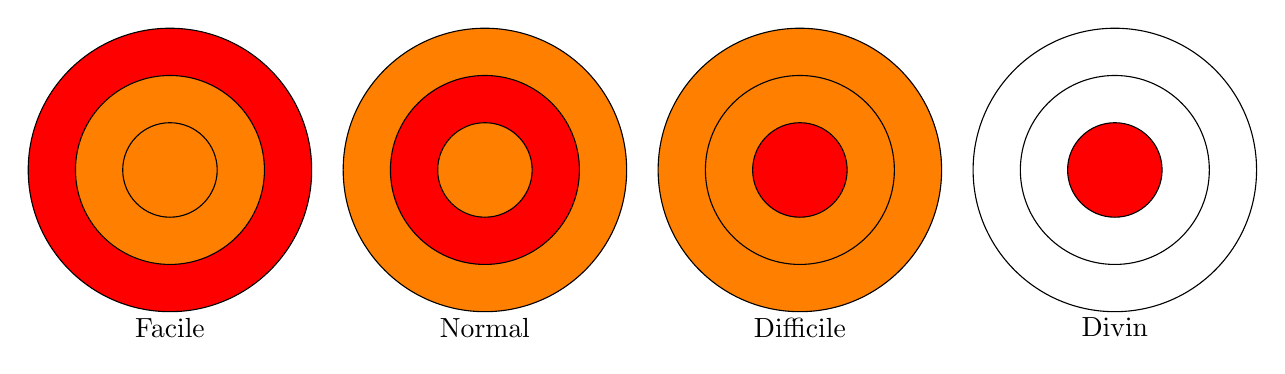
\begin{tikzpicture}
			% facile
			\filldraw[fill=red,draw=black] (-6,0) circle [radius=1.8];
			\filldraw[fill=orange,draw=black] (-6,0) circle [radius=1.2];
			\filldraw[fill=orange,draw=black] (-6,0) circle [radius=0.6];
			\draw (-6,-2) node {Facile};

			% Normal
			\filldraw[fill=orange,draw=black] (-2,0) circle [radius=1.8];
			\filldraw[fill=red,draw=black] (-2,0) circle [radius=1.2];
			\filldraw[fill=orange,draw=black] (-2,0) circle [radius=0.6];
			\draw (-2,-2) node {Normal};

			% Difficile
			\filldraw[fill=orange,draw=black] (2,0) circle [radius=1.8];
			\filldraw[fill=orange,draw=black] (2,0) circle [radius=1.2];
			\filldraw[fill=red,draw=black] (2,0) circle [radius=0.6];
			\draw (2,-2) node {Difficile};

			% Divin
			\filldraw[fill=white,draw=black] (6,0) circle [radius=1.8];
			\filldraw[fill=white,draw=black] (6,0) circle [radius=1.2];
			\filldraw[fill=red,draw=black] (6,0) circle [radius=0.6];
			\draw (6,-2) node {Divin};
		\end{tikzpicture}
	\end{center}
	\caption{Niveaux de difficulté.}
	\label{dif_lvl}
\end{figure}

\begin{figure}
	\begin{center}
		\begin{tikzpicture}[node distance=1.5cm]
			\node[entity] (first) {Connection};
			\node[weak entity] (second) [below of=first] {Choix difficulté} edge (first);
			\node[weak entity] (third) [below of=second] {Choix manches} edge (second);
			\node[relationship] (cond) [below of = third,node distance=2.5cm] {Reste manche ?} edge (third);
			\draw (0.5,-7) node {Oui};
			\draw (1.8,-5.3) node {Non};
			\node[entity] (end) [right of=cond,node distance=3.5cm] {Fin} edge (cond);
			\node[entity] (joueur) [below of=cond,node distance=2.5cm] {Joueur tire} edge (cond);
			\node[entity] (ordi) [below of=joueur] {Robot tire} edge (joueur);
			\draw (0,-10) -- (0,-11);
			\draw (0,-11) -- (-3,-11);
			\draw (-3,-11) -- (-3,-5.5);
			\draw[->] (-3,-5.5) -- (-1.6,-5.5);
		\end{tikzpicture}
	\end{center}
	\caption{Déroulement d'une partie.}
	\label{reg_log}
\end{figure}

\begin{figure}
	\begin{center}
		\includegraphics[scale=0.15]{rc/intro.png}
	\end{center}
	\caption{Le robot.}
	\label{int_rob}
\end{figure}



